\documentclass[10pt]{article}
\usepackage[document]{ragged2e}
\usepackage{multicol}
\usepackage[margin=1in]{geometry}
\usepackage{titlesec}
\usepackage{fancyhdr}
\usepackage{graphicx}
\usepackage{cite}

\pagestyle{fancy}
\fancyhf{}
\fancyfoot[R]{Page. \thepage}
\fancypagestyle{plain}{
    \renewcommand{\headrulewidth}{0pt}
    \fancyhf{}
    \fancyfoot[R]{Page. \thepage}
}

\setlength{\parindent}{0em}
\setlength{\parskip}{1em}
\titlespacing*{\section}{0pt}{0.8em}{0.2em}
\titlespacing*{\subsection}{0pt}{0.2em}{0em}
\titlespacing*{\subsubsection}{0pt}{0.2em}{0em}

\title{
    Towards Real Time Stock Trading \\[.5cm]
    \normalsize MSAI 349 Machine Learning Project Proposal
}
\author{Qingwei Lan}

\begin{document}
\maketitle


\section{Introduction}

Stock markets are marketplaces for buying and selling stocks. Each stock is a piece of ownership of a business. Like all markets, stock markets are dominated by the principles of supply and demand and the core influencers of these principles are the people participating in the stock market trades. In stock markets, most people would envision themselves as completely logical agents. HoIver, the truth is that people are not logical. Human traders are easily influenced by information around them, and the behavior of people will move the market siginificantly.

There are many indicators driving the change in supply / demand in stock markets. In the project, we will devise a neural network using multiple stock analysis indicators as nodes. Furthermore, we will focus on the influence of newly added information on current stock market prices. Specifically we will try to use the publication of news articles to predict how stock prices move, derive buy/sell signals, and devise a general investing strategy based on these signals.

To evaluate our model, we will run our trained model on news articles and stock data on a certain time period not in the training period. We will allocate an imaginary budget of \$1,000,000 to this investing strategy and see how much money we eventually end up with. We will compare this strategy to a baseline ``buy and hold" stragety, for which we will buy stocks at the start of the test period, hold onto them, and determine its valuation at the end of the testing period.

We will run our models on individual stocks like Apple (AAPL), Facebook (FB), Google (GOOG), etc., and on overall stock market index ETFs like the Nasdaq (QQQ), S\&P 500 (SPY), and the Dows Jones Industrial Average (DIA). More details about evaluation can be found in the \textbf{Evaluation} section below.

As a bonus, we might build infrastructure to run this model and predict stock prices in real time with online training, where we will allow our model to continuously update itself based on real time data instead of training only on static data \cite{parisi:2019}.


\section{Data Sources}

The two major sources of data for this project will be stock price data and news data. In the following two sections, we will explore how we fetch data to build our pipeline.

\subsection{Stock Data}

We will access stock data through the following data sources. Most of these are Python libraries with built-in access to the data, however, we may also need to create a web crawler to gather news from sources that don't provide APIs

\begin{enumerate}

\item \textbf{Yahoo Finance (yfinance):} This Python library provides easy access to stock data pulled from the Yahoo Finance website. Its ease of use and quick setup will provide us with good starter information to build our prediction pipeline. It also proivdes high data granularity and is automatically integrated with popular frameworks like Pandas.

\item \textbf{Quandl:} Typically yfinance should provide us with sufficient power to build our pipeline. However, in cases where this might fail, we will use Quandl as a backup data source for getting our stock price data.

\end{enumerate}

\subsection{News Data}

\begin{enumerate}

\item \textbf{Yahoo Financials (yahoofinancials):} This open source Python library provides access to news articles from Yahoo Finance. This API provides us with a simple way to start building our pipeline for stock prediction. However, Yahoo Finance doesn't provide large amounts of news articles, and many of these articles are delayed so we might need to rely on other souces.

\item \textbf{MarketWatch Web Crawler:} We will build a web crawler in Python to crawl the MarketWatch website for latest news articles that are useful for analysis. Specifically, we will gather news information for the individual stocks (and related industry) that we are investing in.

\item \textbf{Twitter Crawler:} We will build a web crawler to gather latest news from Twitter accounts related to the financial market. Typically, Tweets provide real-time access to the latest news and would allow us to make decisions based on real-time sentiment change.

\item \textbf{Reddit Crawler:} Similar to the Twitter Crawler, we will build a crawler to fetch data from Reddit's popular ``wallstreetbets" subreddit. This is an active forum and based on empirical experience, these users are able to cause movements in the market. This data would be useful for building a sentiment analysis model.

\end{enumerate}


\section{Features}

In this section we will describe the main features we will build and how will we use these features to build a neural network for generating stock trading strategies. The main features we will be using are split into fundamental stock indicators, technical stock indicators, and general stock market sentiment. The sections below will describe each of these in detail.

\subsection{Fundamental Indicators}

\subsubsection{Price/Earnings Ratio}

This ratio indicates a company's relative value of each of its shares compared to its earnings. This is a commonly used ratio by stock analysts \cite{fadummies:2016}.

\subsubsection{Earnings per Share}

Earnings per share indicates the profitability of a company. This is usually reported during earnings season and is indicative of how well a company is doing \cite{fadummies:2016}.

\subsection{Technical Indicators}

\subsubsection{Moving Average Convergence Divergence (MACD)}

MACD is short for moving average convergence divergence and measures the trend of stock price movement. It is calculated by subtracting the 26-day exponential moving average from the 12-day exponential moving average. Additionally, a 9-day exponential moving average (signal line) is computed and plotted with the MACD and can be used to generate buy / sell signals. A buy signal is generated when the MACD crosses above its signal line and a sell signal is generated when the MACD crosses under its signal line \cite{tadummies:2020, stankovic:2015, li:2019}.

\subsubsection{Relative Strength Index (RSI)}

The relative strength index (RSI) measures the influence of a recent change in stock price compared to its general trend. It indicates whether a stock is overbought or oversold and is a good indicator for generating buy / sell signals \cite{tadummies:2020, stankovic:2015}.

\subsubsection{On-Balance Volume (OBV)}

On-balance volume is an indicator that measures trading volume's influence on stock price changes. The rationale behind this is that changes in the stock market would accompany volume changes \cite{tadummies:2020}.


\subsection{Stock Market Sentiment Analysis}

We will build a sentiment analysis model using NLP for analyzing news articles and try to predict the general trend of the stock market. We will use this model as a major feature for generating stock buy/sell signals.

More specifically, we want to analyze general sentiment of the stock market (1) for each interested company, (2) for each sector, (3) over time, and (4) sudden changes of sentiment.

The sentiment analysis model will be built as a recurrent neural network (RNN) since we want to track sentiment over time and RNNs are great at processing and modelling such data.


\section{Execution}

In this section, we will describe in detail our execution plan, specifically, (1) how we build our data pipeline, (2) how we build our model with machine learning techniques, and (3) how we evaluate our model. The execution plan is preliminary and may need to evolve as we dive deeper into the project.

\subsection{Data Pipeline Design}

In this project, we are pulling data from multiple data sources, therefore it will be important to make sure we have a stable database with multiple data source components feeding into it.

We will define each data source as an independent component. For example, we will create a \textbf{MarketWatch News} processor that is responsible for downloading news data from the MarketWatch website, cleaning the data, and storing it into database. Similarly, we will have a component for downloading stock price data and storing it into the database. Each of these components should be responsible for handling and reporting failures. This would ensure that the system pipeline is stable and debuggable.

The proposed data pipeline design diagram is shown in Figure \ref{fig:datapipe}.

\begin{figure}[h]
    \centering
    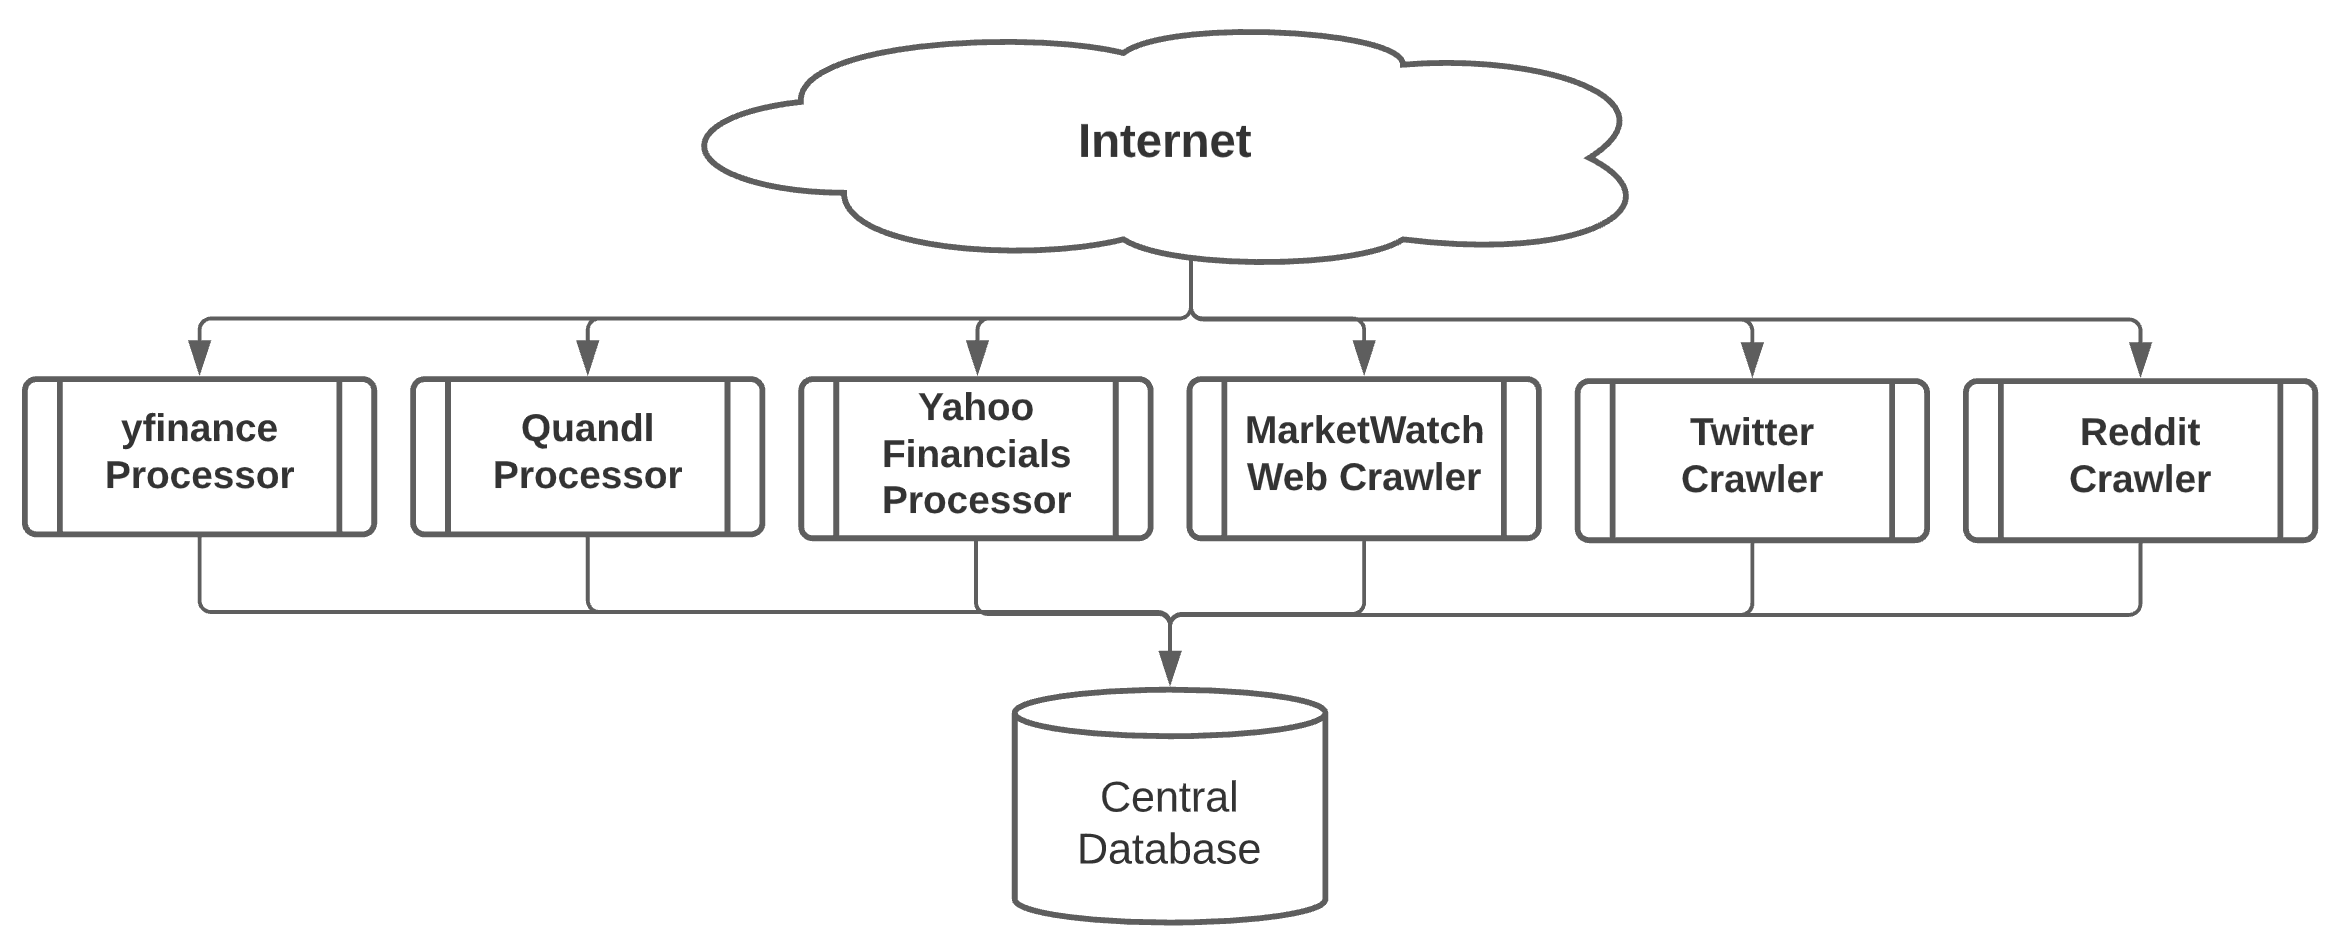
\includegraphics[scale=0.35]{datapipe}
    \caption{Diagram of proposed data pipeline design.}
    \label{fig:datapipe}
\end{figure}

\subsection{Model Generation}

We will first build 5 nodes (features) for the common stock analysis indicators (PE ratio, EPS, MACD, RSI, OBV) and use these as nodes of our neural network. These nodes can be generated directly from stock data. We will train this model to determine how much weight we should assign these nodes.

Next we will build an NLP node (feature) that takes the news data as input and generates a general sentiment analysis as output. This output will be used within the netural network to derive a buy / sell signal.

The overall signal is determined by combining and ranking the output from all feature nodes. We will first train each feature individually. Then we will train the entire neural network will be trained to learn how much weight we should assign to each individual feature.

See Figure \ref{fig:network} for an overview of the proposed neural network.

\begin{figure}[h]
    \centering
    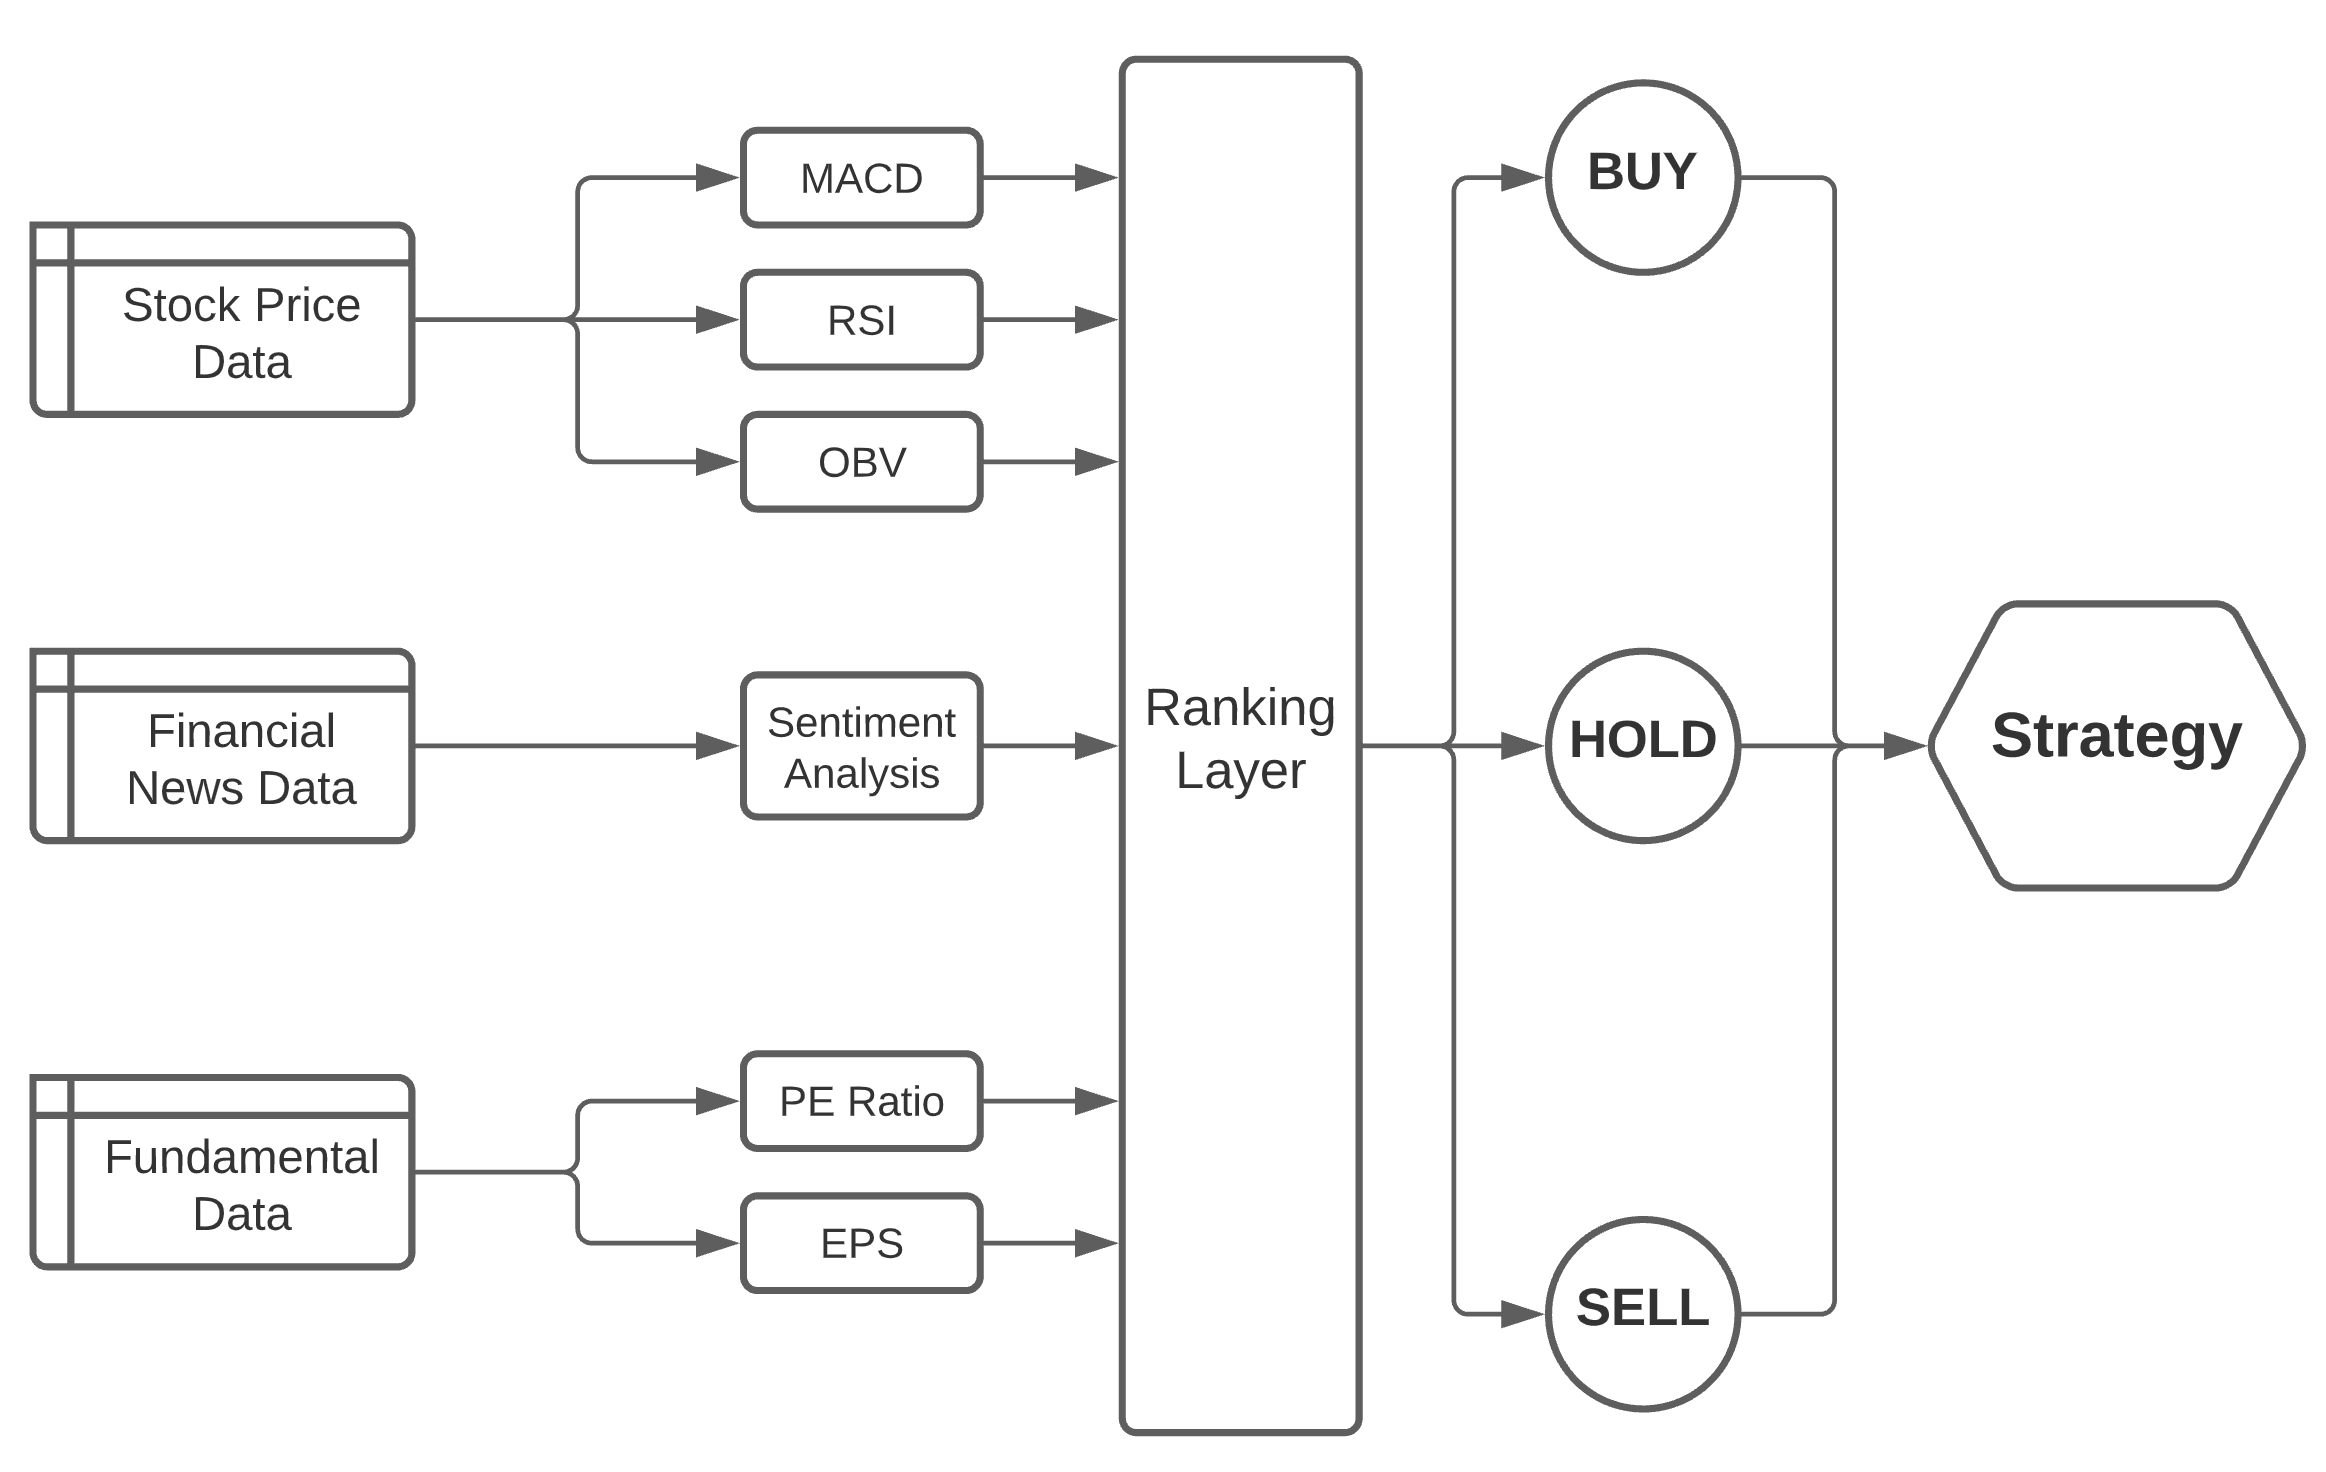
\includegraphics[scale=0.37]{network}
    \caption{Diagram of proposed neural network with features nodes.}
    \label{fig:network}
\end{figure}

\subsection{Evaluation}

We will run two tests, and each test will be run on real data on a certain time period (i.e. one month). For each test, we will have a baseline strategy and a test strategy. At the end of the test period, we will compare the valuation of our test strategy portfolio against the valuation of our baseline strategy portfolio.

As a plus, we might test our strategies on real-time data, but this would depend heavily on how we build our infrastructure to handle real-time continuous streams of data and how we build online training.

\subsubsection{Individual Stocks}

We will choose a few individual stocks to build our model and run our test on. Examples include Apple (AAPL), Facebook (FB), Google (GOOG), etc. In this section, we will run our model on a single stock only. 

Our base strategy is to buy and hold the stock until the end, and we evaluate the final valuation using the closing price at the end of test period.

Our test strategy would allow us to buy and sell the same stock as many times as we want and the final evaluation strategy is to take the sum of the valuation of the stock and any remaining cash we have.

\subsubsection{Stock Market ETFs}

Our baseline strategy is to evenly split our budget between the 3 ETFs (QQQ, SPY, DIA). We will buy the ETFs during the start of our testing period, and hold throughout the period. At the end of the testing period, we will determine the value of the entire portfolio using the closing price on the end date.

Our test strategy is similar to that of individual stocks. The only exception is that we are only allowed to choose from the 3 ETFs (QQQ, SPY, DIA). In the end, we add up all remaining cash (we are allowed to hold cash if our strategy thinks the market is going to go down) and the valuation of all the stocks in our portfolio.

\subsubsection{Dynamic Portfolio}

In this evaluation strategy, we will be running our model on multiple stocks to build a portfolio that tries to maximize profit.

Our baseline strategy is to buy equal valuations of each stock and hold them for the entire testing period.  The final evaluation is the same as that for the ETFs.

For simplicity, our test strategy would allow as many buys and sells as we want (there is no cooldown period or fee associated with each trade). We are allowed to build our portfolio however we want (no restriction on how to allocate our budget), but we are only allowed to buy certain stocks (same stocks as the baseline strategy). The evaluation rules at the end are also the same as that of the ETFs.


\section{Challenges}

The scope of this project is quite large and the following is a list of potential challenges that we might face and how we might address them.

\begin{enumerate}

\item Sentiment analysis on news data would require a lot of data cleaning to ensure the NLP models can understand what the news articles means. Since we are using Twitter data, it might be even more challenging. In this case, we will be starting with simple Yahoo Finance news because it is structured and already cleaned.

\item The amount of stock data is large, and will result in memory pressure during downloading and training. To overcome this, we can download and process the data in batches, save them to a local database such as SQLite or MySQL. During training, we can train our model incrementally to reduce memory pressure.

\item If we want to test our model on real-time data, data might be challenging to retrieve and process. To address this, we will allow some amount of delay during testing, and backtest our model against delayed data. We will try to keep this delay as small as possible.

\end{enumerate}


\bibliographystyle{plain}
\bibliography{refs}

\end{document}
